\section{Question 2}
I think the distribution of passing and failing examples in the data is causing worse performance.  One method for improving the quality of the second network is to train using a different loss function.  Instead of focusing on only on correct classification, adding increased penalty to false positives and false negatives may help the network find a better decision boundary.

\subsection{Part A}
In contrast to the first data set, more hidden units appears to converge faster.  Potentially, because there are many more pass examples than fail examples in this training data set, the smaller network has a hard time finding the decision boundary.  
\begin{figure}[H]
	\centering
	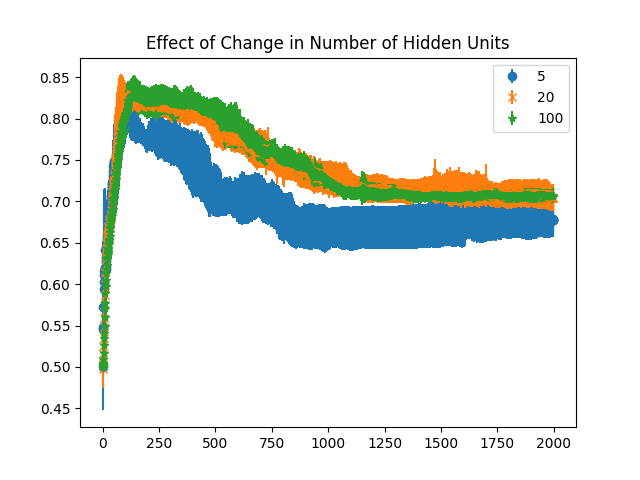
\includegraphics[width=0.6\textwidth]{../train2/hidden_units.png}
	\caption{Effect of changing number of hidden units}
\end{figure}

\subsection{Part B}
Similar to the first data set, at some point, training causes overfitting to the training set and performance on the test set decreases.  However, the time for convergence is much longer for this data set as compared to the first data set.  200 epochs appears to be insufficient to reach convergence.
\begin{figure}[H]
	\centering
	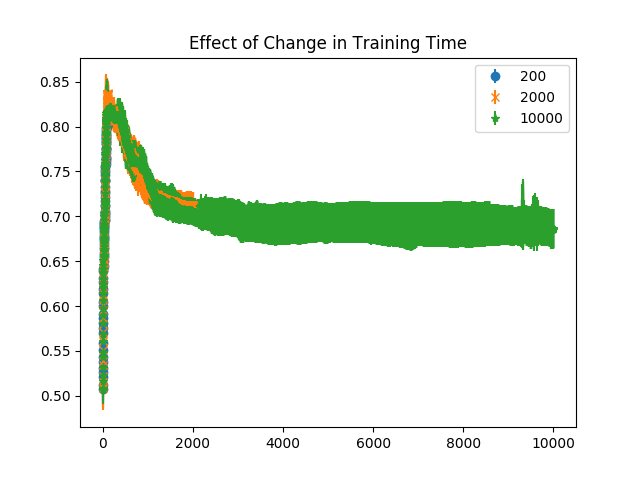
\includegraphics[width=0.6\textwidth]{../train2/epochs.png}
	\caption{Effect of changing traning time}
\end{figure}

\subsection{Part C}
Learning rate has a similar effect as for the first data set.  In this case, the very small learning rate appears to be unable to find a good solution.  It appears to get stuck in a terrible solution which predicts the same value every time.  
\begin{figure}[H]
	\centering
	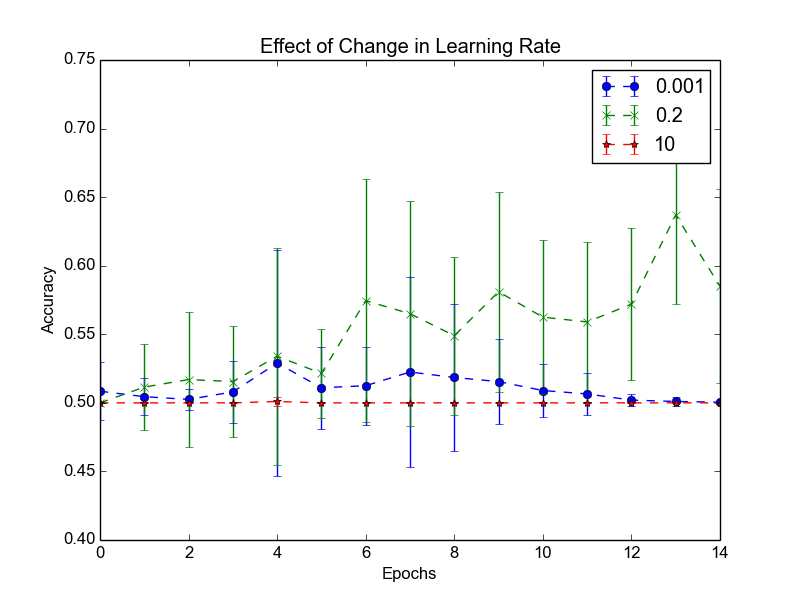
\includegraphics[width=0.6\textwidth]{../train2/learning_rate.png}
	\caption{Effect of changing learning rate}
\end{figure}

\subsection{Part D}
I examined how initialization of the weights affects the algorithm.  The legend shows the magnitude of the initial values.  The results are similar to the first data set.  Too large and the network saturates and too small and the network is unable to learn. 
\begin{figure}[h]
	\centering
	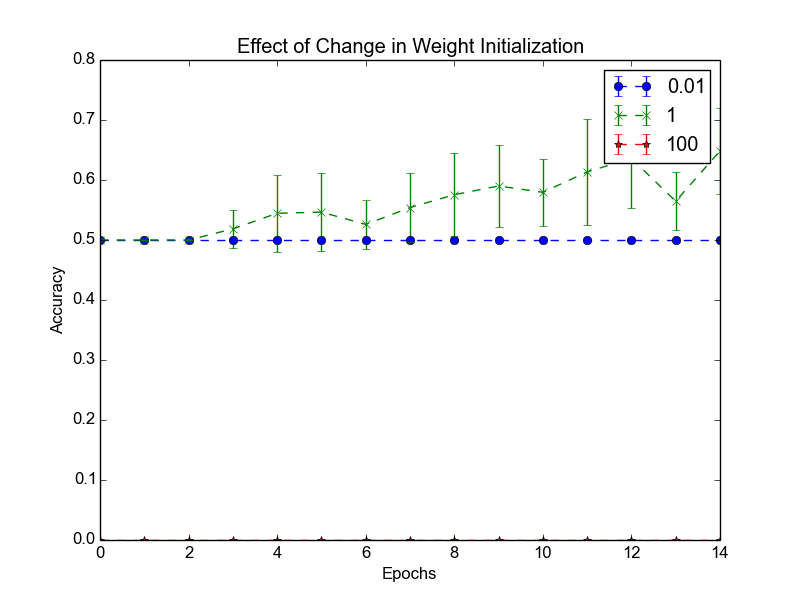
\includegraphics[width=0.6\textwidth]{../train2/weights.png}
	\caption{Effect of classifier on different test data sets}
\end{figure}

\subsection{Part E}
The second network seems to excel where the first network struggles, but overall has worse average performance across all the data sets.  The number of passing and failing examples in the second test set is most similar to the second training set.  Due to the similarity, the network performs well on the second test set.  The first test set has an even number of passing and failing examples and the performance is average.  The third data set has mostly passing examples.  The large difference in the distribution of passing and failing examples causes the network to predict poorly.  
\begin{figure}[H]
	\centering
	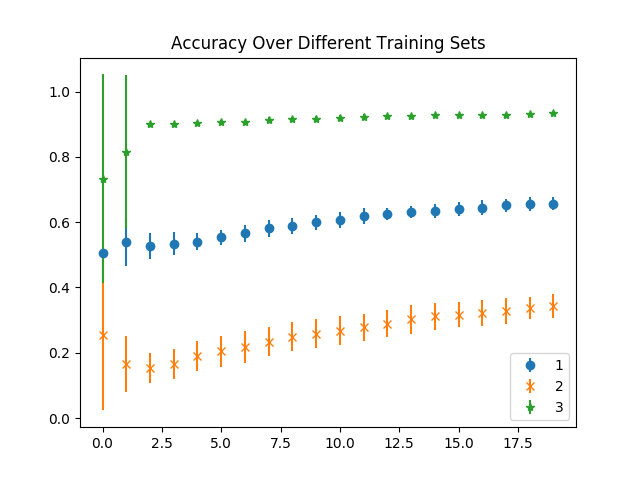
\includegraphics[width=0.6\textwidth]{../train2/data_sets.png}
	\caption{Effect of classifier on different test data sets}
\end{figure}